\documentclass[11pt,a4paper]{article}
\usepackage[margin=2.2cm]{geometry}
\usepackage{amsmath,amssymb}
\usepackage{booktabs}
\usepackage{graphicx}
\usepackage{caption}
\usepackage{hyperref}
\usepackage{xcolor}
\usepackage{enumitem}
\usepackage{microtype}
\usepackage{placeins}
\hypersetup{colorlinks=true,linkcolor=blue!60!black,citecolor=blue!60!black,urlcolor=blue!60!black}
\graphicspath{{../figures/}}
\setlist{nosep}

\title{AI6124 Assignment 2 \\ \large Cancer-versus-Non-Cancer Classification with ROC and Equal-Error-Rate Analysis}
\author{Hanny | Matric Number: G1234567X}

\begin{document}
\maketitle

\begin{abstract}
This report builds a supervised cancer-versus-non-cancer decision tool on the NUH ovarian blood-assay data, determines the decision boundary that best equalizes the two error rates, and plots the ROC (receiver operating characteristic) curve traced by sweeping that boundary; the Wisconsin Diagnostic Breast Cancer (WDBC) data serve as a lower-variance check. Eight classifiers are compared while few more are examined. The main NUH target treats borderline tumours as screening-positive alongside invasive cancers, a conservative choice given that a false negative is the less acceptable error, and one that is tested explicitly rather than assumed. Selecting on training OOF (out-of-fold) scores alone, random forest is chosen; its OOF threshold of $0.484$ yields test FPR/FNR of $0.214/0.231$ on the untouched test split, and a pooled cross-validation over all cases ranks the same model first as a stability check rather than a held-out estimate. Reassigning or excluding borderline cases moves that CV EER to approximately $0.20$, so the result is conditional on the label convention. WDBC is near saturation (test AUC $0.977$--$0.997$). A third data set, SUPPORT2 (9105 cases), is for an intermediate difficulty tier, and is where the methods separate.
\end{abstract}

\section{Task and Decision Criterion}
The task is to learn a binary supervised classifier, determine the boundary that best balances false positives and false negatives, and plot the ROC curve obtained by varying that boundary. Each model returns a score $s(\mathbf{x})$ and predicts the positive class when $s(\mathbf{x})\ge\theta$. The scalar \emph{threshold} $\theta$ induces the feature-space \emph{decision boundary} $\{\mathbf{x}:s(\mathbf{x})=\theta\}$.

Sweeping $\theta$ traces the ROC curve, with false-positive rate $\mathrm{FPR}(\theta)$ and true-positive rate $\mathrm{TPR}(\theta)$. The false-negative rate is $\mathrm{FNR}=1-\mathrm{TPR}$, and the equal error rate is the intersection with $\mathrm{FPR}=\mathrm{FNR}$. Area under the ROC curve (AUROC, abbr. AUC in this report as this report does not use AUPRC) measures ranking performance independently of a single threshold.

An empirical ROC curve is stepwise. I report an interpolated EER, marked by an asterisk in the tables, but do not imply that its exact intersection is always attainable by one deterministic threshold. My threshold is selected separately from training out-of-fold (OOF) scores as the empirical ROC threshold that minimises $|\mathrm{FPR}-\mathrm{FNR}|$, using the lower balanced error as a tie-breaker. Test-set EERs are descriptive only and are not used for model or threshold selection.

\section{Data}
\subsection{NUH ovarian blood assays}
The NUH data accompany the ovarian-cancer study of Tan \emph{et al.}~\cite{tan2008}. The supplied group \texttt{g2} files contain 28 blood-assay features. Inspection shows that \texttt{c1}--\texttt{c4} are one-vs-rest labels of the same patients rather than cross-validation folds: borderline, benign/normal, Stage I--II, and Stage III--IV, respectively. Three borderline test rows duplicate training rows and are removed, leaving 55 training cases and 54 test cases. Across the retained data there are 5 borderline, 56 benign/normal, 14 Stage I--II, and 34 Stage III--IV cases.

The main screening target is \textbf{positive = borderline $\cup$ Stage I--IV} and \textbf{negative = benign/normal}, giving 53 positive and 56 negative cases. Borderline ovarian tumours are not synonymous with invasive malignancy; grouping them with the positive class is a conservative screening decision intended to avoid a potentially consequential false negative. Section~\ref{sec:borderline} reports how the results change when borderline cases are excluded or assigned to the negative class.

Feature identities cannot be mapped reliably because the file column order does not match the source paper I found; they are therefore denoted $f_1,\ldots,f_{28}$. On the training set, $f_{23}$, $f_{24}$ and $f_{28}$ have maximum-to-median ratios above 20. These columns are transformed by $\log(1+x)$ before standardisation; the transformation and scaler are fitted inside each training fold.

\subsection{Wisconsin Diagnostic Breast Cancer}
WDBC contains 569 fine-needle aspirates with 30 nuclear-morphology features, comprising 212 malignant and 357 benign cases~\cite{bcwd,wdbc}. A stratified 80/20 split with seed 0 gives 455 training cases and 114 test cases. The data are close to linearly separable and are used as a sanity check rather than another clinical claim.

\subsection{SUPPORT2}
\label{sec:support2-data}
The two data sets above sit at opposite ends of what a ROC comparison can resolve. NUH has 109 cases, so the fold-wise spread is wider than the gaps between models; WDBC puts every model above AUC $0.97$, so the curves coincide for a different reason. Neither regime lets one read off how the learning rules actually differ. SUPPORT2 is added to fill the gap between them, and is chosen for that operating regime rather than for any resemblance to the tumour task: it is not an oncology data set and carries no clinical claim here.

The target is in-hospital death among seriously ill hospitalised adults, from the SUPPORT study~\cite{knaus1995,support2uci}: 9105 patients, $25.9\%$ positive, with mixed continuous and categorical fields and up to $53\%$ missingness in individual columns. Predictors are the demographics, comorbidity and physiology recorded on study entry, including the SUPPORT and APACHE severity scores. Fifteen columns are removed as identifiers or post-hoc records --- anything billed, scored, or observed at or after discharge, such as total costs, length of stay, time to death, two-month functional status, and resuscitation orders --- because using them would presuppose the outcome. Categorical fields are one-hot encoded with missing as its own level, which is a fixed schema rather than a fitted statistic and so cannot leak; missing numeric values are median-imputed by the same in-fold pipeline that fits the scaler. This leaves 47 features, split stratified 80/20 with seed 0 into 7284 training and 1821 test cases.

\section{Models}
Twelve models were implemented and run under the identical protocol on all three data sets; the eight reported here are a representative subset spanning the linear, kernel, ensemble, neural, fuzzy, and pre-trained families. The four omitted models (an extreme learning machine, MLP-PC, MLP-GA, and a LightGBM gradient-boosting ensemble) are retained in my code, and including them does not change the selected model on any data set.

Logistic regression ($L_2$, $C=1$), an RBF-SVM, and two tree ensembles --- a 500-tree random forest and LightGBM gradient boosting, both left untuned so that the two ensembles are compared on equal terms --- provide the linear, kernel and ensemble baselines. The SVM selects $C\in\{0.1,1,10,100\}$ and $\gamma\in\{\text{scale},0.01,0.1\}$ by inner 5-fold AUC.

A $d$-64-32-1 multilayer perceptron (MLP) with $\tanh$ hidden units is trained for 300 full-batch epochs using Adam (learning rate $10^{-3}$, weight decay $10^{-3}$); this is \textbf{MLP-BP}, back-propagation being the learning rule. Several models keep that feed-forward core and change only how its weights are found, so they are named \textbf{MLP-\emph{rule}} throughout: \textbf{MLP-FF} trains each layer on a local goodness objective over label-embedded positive and negative examples, with no error signal flowing backwards~\cite{ff2022}; \textbf{MLP-CMA-ES} optimises the same parameter vector without gradients using separable CMA-ES (population 32, 300 generations)~\cite{hansen}; and the two models not reported here, \textbf{MLP-PC} (predictive coding) and \textbf{MLP-GA} (a real-coded genetic algorithm), follow the same convention. MLP-FF is the one loose fit: it needs ReLU units and two extra label inputs, so it matches the others in depth and width rather than exactly.

The fuzzy model is a four-rule first-order Takagi--Sugeno ANFIS with Gaussian membership functions and scatter-partition initialisation~\cite{jang1993}. TabPFN v3 (package version 8.4.0)~\cite{tabpfnv3} is included as a strong pre-trained tabular reference; it performs in-context prediction without task-specific gradient training, following the prior-fitted-network formulation introduced by Hollmann \emph{et al.}~\cite{tabpfn}.
\section{Evaluation protocol}
Every decision is made on training data, and the test split is used once, only to report. Concretely, for the given NUH and WDBC splits, preprocessing is fitted on training data only, and 5-fold CV \emph{within the training set} produces OOF scores. Both the choice of model and the choice of threshold are made from those training-OOF scores. The model is then refitted on the complete training set and evaluated once on the test set; the test AUC, interpolated test EER, and the operating point of the selected model are reported afterwards and feed back into nothing.

A separate, purely descriptive summary is also reported. A 54-case test split makes any single estimate volatile, so all cases are additionally evaluated by $5\times$ repeated stratified 5-fold CV (25 fits per model), with the preprocessing refitted inside each fold. These pooled CV columns are computed over the whole cohort and therefore \emph{include the test cases}; they are a resampling summary of how stable a model is across partitions of the available data, not a held-out estimate, and they are not used to select the model, the threshold, or the label policy. Where the pooled ranking is quoted below it is descriptive only, and the selection it would imply is stated separately.

Repeating the split five times is what a small cohort needs; SUPPORT2 does not need it. With 9105 cases a single stratified 5-fold pass already gives fold-wise spreads near $\pm0.01$ AUC, against $\pm0.07$ on NUH, so repeating it would refine a quantity that is already stable at the third decimal. SUPPORT2 is therefore run at 11 fits per model rather than 31. Everything else --- the in-training 5-fold OOF scores, the threshold rule, and the single use of the test split --- is identical across all three data sets.

All experiments use seed 0 on CPU. The reproduced environment is Python 3.13.5, scikit-learn 1.9.0, PyTorch 2.13.0, \texttt{cma} 4.4.4, and TabPFN 8.4.0.

\section{Results}
\subsection{NUH main screening analysis}
Table~\ref{tab:nuh} orders models by the pooled repeated-CV results; Figure~\ref{fig:nuh-roc} shows the test ROC curves. Random forest has the highest pooled CV AUC ($0.845\pm0.066$) and the lowest pooled CV EER ($0.245\pm0.089$), followed by TabPFN on both metrics. As stated in Section~4, these pooled columns include the test cases and are reported to show stability, not to choose a model; the fold-wise spreads are in any case larger than most differences between methods (Figure~\ref{fig:cv-paired}), so the ordering is descriptive.

\begin{table}[htbp]
\centering\small
\caption{NUH-g2 main screening label (borderline positive). Test EER$^{*}$ is the interpolated ROC intersection. CV columns are $5\times5$ repeated-CV over all 109 cases (mean $\pm$ fold-wise s.d.); because they pool the training and test cases they are a stability summary, not a held-out estimate, and the model was selected on training-OOF scores instead (Section~4).}
\label{tab:nuh}
\setlength{\tabcolsep}{8pt}
\begin{tabular}{lcccc}
\toprule
Model & Test AUC & Test EER$^{*}$ & CV AUC & CV EER \\
\midrule
LogReg & 0.691 & 0.346 & 0.773 $\pm$ 0.083 & 0.272 $\pm$ 0.083 \\
SVM-RBF & 0.805 & 0.250 & 0.809 $\pm$ 0.085 & 0.282 $\pm$ 0.091 \\
RandomForest & 0.789 & 0.231 & \textbf{0.845 $\pm$ 0.066} & \textbf{0.245 $\pm$ 0.089} \\
MLP-BP & 0.640 & 0.357 & 0.764 $\pm$ 0.083 & 0.286 $\pm$ 0.074 \\
MLP-FF & \textbf{0.820} & 0.269 & 0.813 $\pm$ 0.082 & 0.272 $\pm$ 0.090 \\
MLP-CMA-ES & 0.746 & 0.231 & 0.801 $\pm$ 0.073 & 0.269 $\pm$ 0.063 \\
ANFIS & 0.673 & 0.385 & 0.749 $\pm$ 0.121 & 0.302 $\pm$ 0.108 \\
TabPFN & 0.765 & 0.250 & 0.828 $\pm$ 0.064 & 0.255 $\pm$ 0.076 \\
\bottomrule
\end{tabular}
\end{table}

\begin{figure}[htbp]
\centering
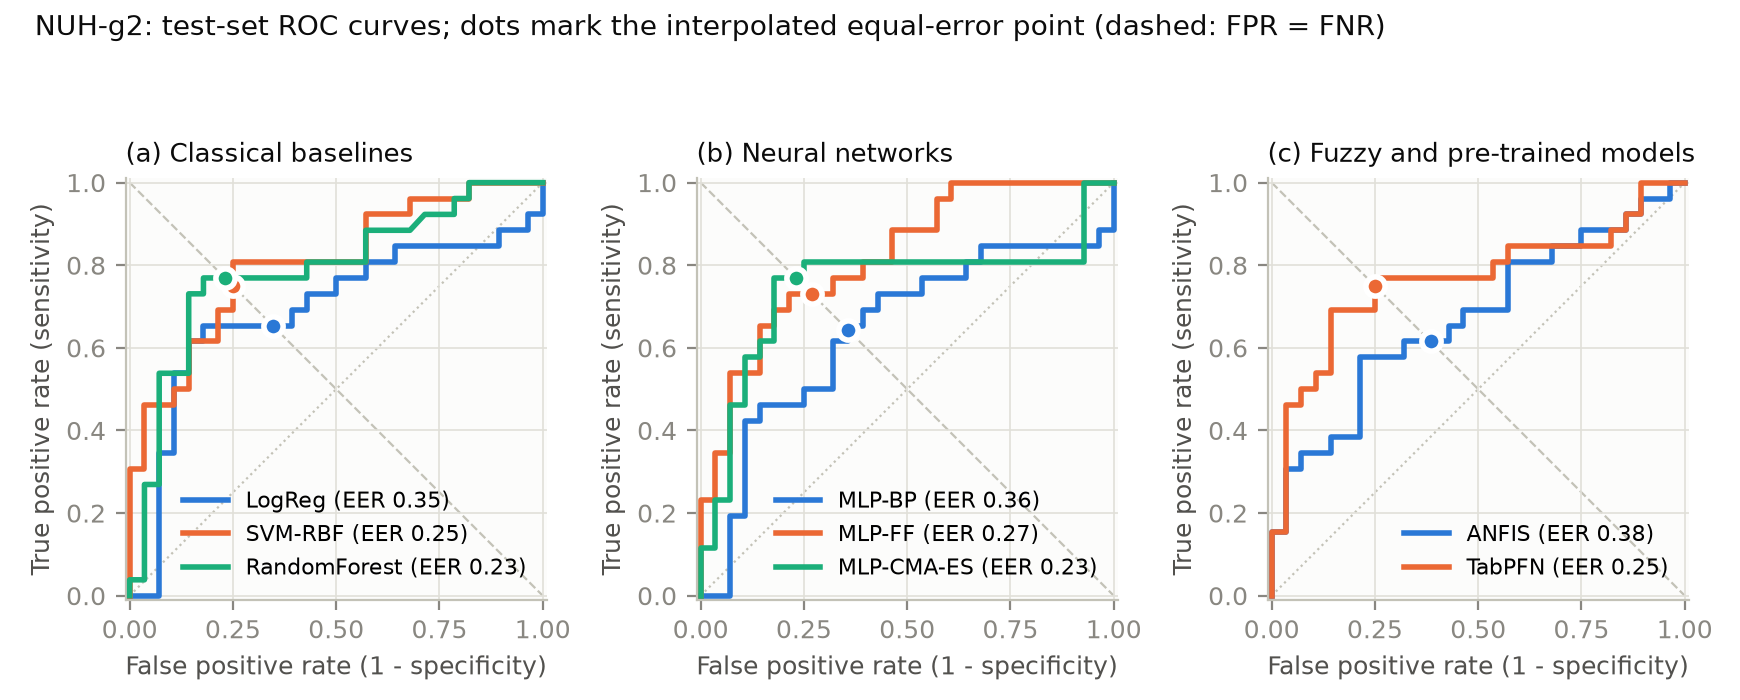
\includegraphics[width=\textwidth]{nuh_roc_focused.png}
\caption{NUH test ROC curves for the reported model set, one panel per model family. Dots mark linearly interpolated EER points; a dot can lie between two empirical operating points and need not correspond to one deterministic threshold.}
\label{fig:nuh-roc}
\end{figure}

\begin{figure}[htbp]
\centering
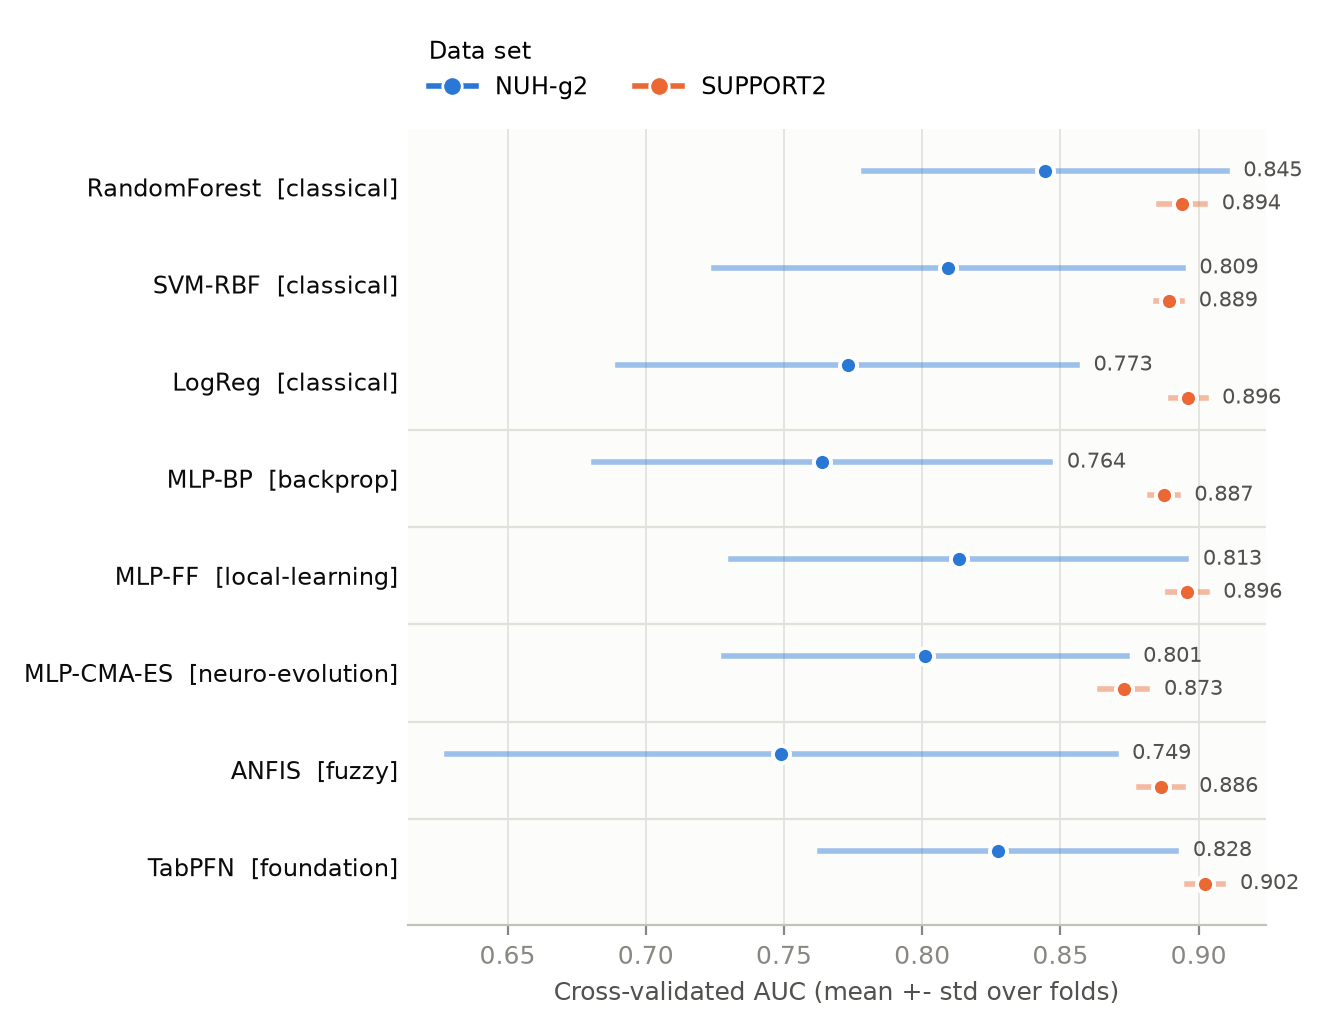
\includegraphics[width=0.86\textwidth]{cv_auc_nuh_support2.png}
\caption{Cross-validated AUC per model, both data sets on one model axis. \textcolor[HTML]{2A78D6}{\textbf{Blue}} is NUH-g2 (pooled $5\times5$ CV over all 109 cases, mean $\pm$ fold-wise s.d.); \textcolor[HTML]{EB6834}{\textbf{orange}} is SUPPORT2 (single 5-fold pass over all 9105 cases). Rows are ordered by the NUH value within each model family. The NUH intervals overlap substantially, so the ordering in Table~\ref{tab:nuh} is descriptive rather than evidence of a reliable difference between methods; the SUPPORT2 intervals are roughly an order of magnitude tighter, which is what makes the ranking in Table~\ref{tab:support2} readable. As in Table~\ref{tab:nuh}, both series pool training and test cases and neither was used for selection.}
\label{fig:cv-paired}
\end{figure}

\paragraph{Selected decision boundary.}
Model selection uses the training-OOF scores alone: neither the test set nor the pooled CV columns take part. On the training OOF scores random forest is best on both criteria (AUC $0.812$, EER $0.236$; next best TabPFN, $0.796$ and $0.250$), so it is selected, and its closest attainable training-OOF equal-error threshold is $\theta_{\mathrm{OOF}}=0.484$ on the vote fraction. Applied after refitting, this threshold gives test FPR $0.214$, FNR $0.231$, sensitivity $0.769$, specificity $0.786$, and accuracy $0.778$; the interpolated test EER is $0.231$. MLP-CMA-ES happens to reach the same descriptive test EER, but it was not selected: its training-OOF EER is clearly worse ($0.296$), and the test-set values were not available to the selection step. That the pooled CV ranking in Table~\ref{tab:nuh} also puts random forest first is a consistency check reported after the fact, not the reason for the choice.

The second tree ensemble makes the same point from the other side. LightGBM reaches training-OOF AUC $0.758$ and EER $0.296$, well behind the random forest, so it is not selected --- yet it looks better under both of the views the protocol excludes, with pooled CV EER $0.233$ against $0.245$ and a tied test EER of $0.231$. Selecting on either would have changed the answer, on quantities that include the test cases.

\FloatBarrier
\subsection{Sensitivity to the borderline label}
\label{sec:borderline}
The source data distinguish borderline tumours from both benign/normal cases and invasive cancer. I therefore repeat the pooled $5\times5$ CV for SVM-RBF, random forest, and MLP-BP under three policies: borderline as screening-positive (main analysis), excluded, and assigned to non-cancer. This comparison is deliberately run on the pooled cohort, because the question is how the \emph{target definition} changes the achievable error rate rather than how one fitted model generalises; for the same reason the numbers below are not held-out estimates and none of them was used to choose the reported model or its threshold.

\begin{table}[htbp]
\centering\footnotesize
\caption{NUH borderline-label sensitivity. Counts are retained total cases with cancer/non-cancer counts in parentheses.}
\label{tab:borderline}
\setlength{\tabcolsep}{7pt}
\begin{tabular}{llccc}
\toprule
Borderline policy & Model & $n$ (cancer/non-cancer) & CV AUC & CV EER \\
\midrule
Cancer & SVM-RBF & 109 (53/56) & 0.809 $\pm$ 0.085 & 0.282 $\pm$ 0.091 \\
Cancer & RandomForest & 109 (53/56) & 0.845 $\pm$ 0.066 & 0.245 $\pm$ 0.089 \\
Cancer & MLP-BP & 109 (53/56) & 0.764 $\pm$ 0.083 & 0.286 $\pm$ 0.074 \\
Excluded & SVM-RBF & 104 (48/56) & 0.828 $\pm$ 0.078 & 0.250 $\pm$ 0.095 \\
Excluded & RandomForest & 104 (48/56) & 0.882 $\pm$ 0.065 & 0.195 $\pm$ 0.082 \\
Excluded & MLP-BP & 104 (48/56) & 0.762 $\pm$ 0.091 & 0.282 $\pm$ 0.092 \\
Non-cancer & SVM-RBF & 109 (48/61) & 0.832 $\pm$ 0.086 & 0.243 $\pm$ 0.077 \\
Non-cancer & RandomForest & 109 (48/61) & 0.885 $\pm$ 0.066 & 0.196 $\pm$ 0.082 \\
Non-cancer & MLP-BP & 109 (48/61) & 0.779 $\pm$ 0.104 & 0.256 $\pm$ 0.120 \\
\bottomrule
\end{tabular}
\end{table}

The policy materially changes the point estimates: for random forest, excluding borderline cases moves CV AUC/EER from $0.845/0.245$ to $0.882/0.195$, and assigning them to non-cancer gives $0.885/0.196$; SVM and MLP-BP move the same way. This is consistent with borderline cases being hard to separate from benign ones~\cite{tan2008}, but the fold-wise spreads overlap and only five borderline patients are involved, so the experiment shows sensitivity to the target definition without establishing that any policy is clinically preferable. The screening-positive policy is retained as the more conservative choice when false negatives are the more serious error.

\FloatBarrier
\subsection{WDBC sanity check}
All reported models perform strongly on WDBC (Table~\ref{tab:wdbc}): test AUC ranges from $0.977$ to $0.997$, rather than being strictly above $0.98$ for every model. TabPFN has the best test AUC ($0.997$), interpolated test EER ($0.024$), pooled CV AUC ($0.997\pm0.004$), and pooled CV EER ($0.023\pm0.019$). WDBC is used only as an implementation check, so no model is selected on it and these figures are reported descriptively; the near-saturated results confirm that the ROC/EER pipeline behaves as expected on a larger, well-conditioned data set.

\begin{table}[htbp]
\centering\small
\caption{WDBC results. Definitions are the same as in Table~\ref{tab:nuh}.}
\label{tab:wdbc}
\setlength{\tabcolsep}{8pt}
\begin{tabular}{lcccc}
\toprule
Model & Test AUC & Test EER$^{*}$ & CV AUC & CV EER \\
\midrule
LogReg & 0.993 & 0.048 & 0.995 $\pm$ 0.005 & 0.029 $\pm$ 0.020 \\
SVM-RBF & 0.994 & 0.048 & 0.996 $\pm$ 0.006 & 0.028 $\pm$ 0.022 \\
RandomForest & 0.977 & 0.048 & 0.990 $\pm$ 0.009 & 0.041 $\pm$ 0.021 \\
MLP-BP & 0.989 & 0.071 & 0.995 $\pm$ 0.006 & 0.032 $\pm$ 0.019 \\
MLP-FF & 0.988 & 0.069 & 0.994 $\pm$ 0.008 & 0.028 $\pm$ 0.017 \\
MLP-CMA-ES & 0.984 & 0.069 & 0.994 $\pm$ 0.008 & 0.032 $\pm$ 0.020 \\
ANFIS & 0.992 & 0.048 & 0.994 $\pm$ 0.006 & 0.030 $\pm$ 0.019 \\
TabPFN & 0.997 & 0.024 & \textbf{0.997 $\pm$ 0.004} & \textbf{0.023 $\pm$ 0.019} \\
\bottomrule
\end{tabular}
\end{table}

\FloatBarrier
\subsection{SUPPORT2}
\label{sec:support2-results}
Table~\ref{tab:support2} and Figure~\ref{fig:support2-roc} give the SUPPORT2 results. The whole field falls inside a CV AUC band of $0.873$--$0.902$, a span of $0.029$, against a fold-wise spread of about $\pm0.007$: small differences, but for the first time larger than the noise, which is the point of adding this tier. Three things follow, all of them about the models rather than about the data.

\begin{table}[htbp]
\centering\small
\caption{SUPPORT2 results (in-hospital death, 9105 cases). Definitions are the same as in Table~\ref{tab:nuh}, except that the CV columns are a single stratified 5-fold pass over all cases rather than $5\times5$ repeats (Section~4). As on WDBC, no model is selected on this data set.}
\label{tab:support2}
\setlength{\tabcolsep}{8pt}
\begin{tabular}{lcccc}
\toprule
Model & Test AUC & Test EER$^{*}$ & CV AUC & CV EER \\
\midrule
LogReg & 0.892 & 0.186 & 0.896 $\pm$ 0.006 & 0.183 $\pm$ 0.010 \\
SVM-RBF & 0.883 & 0.191 & 0.889 $\pm$ 0.005 & 0.186 $\pm$ 0.005 \\
RandomForest & 0.887 & 0.189 & 0.894 $\pm$ 0.008 & 0.179 $\pm$ 0.007 \\
MLP-BP & 0.879 & 0.201 & 0.887 $\pm$ 0.005 & 0.192 $\pm$ 0.006 \\
MLP-FF & 0.891 & 0.187 & 0.896 $\pm$ 0.007 & 0.179 $\pm$ 0.008 \\
MLP-CMA-ES & 0.862 & 0.208 & 0.873 $\pm$ 0.009 & 0.199 $\pm$ 0.013 \\
ANFIS & 0.887 & 0.190 & 0.886 $\pm$ 0.008 & 0.192 $\pm$ 0.008 \\
TabPFN & 0.897 & 0.181 & \textbf{0.902 $\pm$ 0.007} & \textbf{0.176 $\pm$ 0.007} \\
\bottomrule
\end{tabular}
\end{table}

\begin{figure}[htbp]
\centering
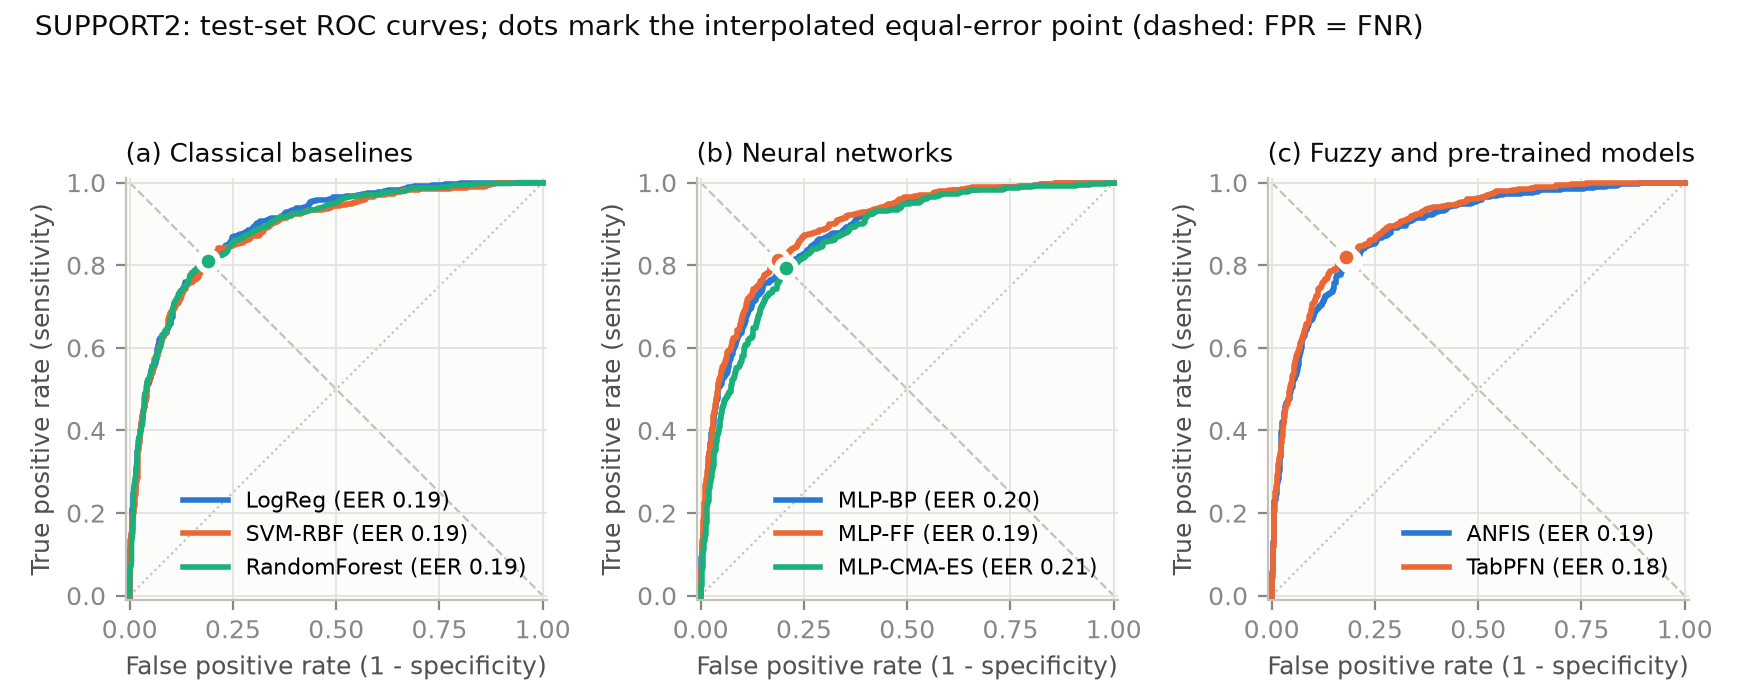
\includegraphics[width=\textwidth]{support2_roc_focused.png}
\caption{SUPPORT2 test ROC curves for the reported model set, one panel per model family, drawn on the same convention as Figure~\ref{fig:nuh-roc}. With 1821 test cases the curves are smooth, so the interpolated equal-error point is close to an attainable threshold.}
\label{fig:support2-roc}
\end{figure}

First, logistic regression is not beaten by much. At CV AUC $0.896\pm0.006$ it is level with MLP-FF at the head of the locally trained models --- the two differ by $0.0003$ --- and ahead of random forest, SVM-RBF, MLP-BP and ANFIS; only TabPFN ($0.902\pm0.007$) is above it. Whatever structure the extra capacity could exploit is mostly not there, so on this data set the ranking rewards regularisation rather than expressiveness.

Second, the learning rule matters more than the architecture, and it changes sign with sample size. MLP-BP, MLP-FF, MLP-PC and MLP-CMA-ES share the same $d$-64-32-1 core and differ only in how the weights are found, yet they span $0.873$ to $0.896$. MLP-CMA-ES is last on both metrics, whereas on NUH the same model was \emph{ahead} of MLP-BP ($0.801$ against $0.764$). Gradient-free search over roughly $6\times10^3$ weights is competitive when 109 cases make gradients noisy, and falls behind once 9105 cases make them reliable. MLP-FF is the opposite case: layer-local learning gives up nothing here, matching logistic regression to three decimals.

Third, the cost ordering has nothing to do with the accuracy ordering. One MLP-BP fit takes $12.7$\,s; MLP-CMA-ES takes $289.6$\,s for a worse model, and TabPFN takes $548.8$\,s, almost all of it in prediction rather than fitting, since it does no task-specific training. 
TabPFN also refuses more than 5000 rows at CPU unless an override is set, so the best model here is the one that needed its own guard rail disabled to run at all --- worth re-thinking against a $0.006$ AUC lead over a logistic regression that fits in $0.18$\,s, as Dr.Wang said at the third lecture, ``\emph{Don't kill a chicken with a knife for killing bulls}''.

\section{Discussion}
The core assignment requirements are satisfied: each classifier produces a continuous score, ROC curves are generated by sweeping the decision threshold, and the selected random-forest boundary is determined exclusively from training OOF predictions. Separating the interpolated EER from the attainable threshold avoids claiming an exact FPR--FNR equality that a finite test set cannot necessarily realise.

The NUH results are dominated by small-sample uncertainty and label definition. The training-OOF comparison supports random forest as the preferred choice under the stated protocol, and the pooled CV agrees, but neither shows that the alternative learning rules are equivalent or non-inferior: every ranking sits inside the fold-wise spread. Separating the methods therefore needs the third data set, where the spread is roughly ten times smaller than the same differences. What appears there is about the methods, not about ovarian cancer --- a linear model is hard to beat, layer-local learning costs nothing, and gradient-free weight search is the one approach that clearly degrades as the sample grows, which is invisible at $n=109$, where the same optimiser looked competitive.

The EER objective gives false positives and false negatives equal weight, as required by the task. A clinical screening threshold would normally favour sensitivity and must be chosen using explicit costs, prevalence, and clinical validation. Treating borderline cases as screening-positive addresses the label side of that concern but does not replace cost-sensitive threshold selection.

Limitations include the five borderline cases, the reverse-engineered NUH file structure, fixed hyperparameters for most models, and reliance on one local version stack. TabPFN additionally requires licensed weights. Exact dependency versions and data checksums should be retained with the submitted code because an unpinned package list alone is insufficient for long-term reproduction.

\section{Conclusion}
Random forest is the preferred decision tool for the main NUH screening definition. It was selected on training-OOF scores alone (OOF AUC $0.812$, OOF EER $0.236$), and its training-OOF vote threshold of $0.484$ yields $0.769$ sensitivity and $0.786$ specificity on the test split, which was held out from both the model choice and the threshold choice. The pooled CV ranks the same model first but is a stability check, not an out-of-sample estimate. The ROC analysis satisfies the requested decision-boundary sweep, and WDBC provides a successful implementation check. On SUPPORT2, added only to obtain a regime in which the methods are distinguishable, the ordering is narrow but stable: TabPFN first at CV AUC $0.902\pm0.007$, logistic regression next at $0.896\pm0.006$ for a fraction of the compute, and gradient-free MLP training last. Most importantly, the borderline sensitivity experiment shows that NUH performance estimates depend materially on whether five clinically ambiguous cases are treated as positive, excluded, or treated as negative. The reported result is therefore conditional on the explicitly stated conservative screening label.

\section{AI Usage Disclosure}
This assignment was written by the student, with the assistance of AI tools (ChatGPT and Claude) for grammar, style checking and code generation. The student has verified that all content is original and that any AI-generated suggestions have been critically evaluated and appropriately integrated.

\begingroup\small
\begin{thebibliography}{9}
\bibitem{tan2008} T.~Z. Tan, C. Quek, G. S. Ng, K. Razvi. Ovarian cancer diagnosis with complementary learning fuzzy neural network. \emph{Artificial Intelligence in Medicine} 43:207--222, 2008.
\bibitem{bcwd} W. Wolberg, O. Mangasarian, N. Street, W. Street. Breast Cancer Wisconsin (Diagnostic) [Dataset]. UCI Machine Learning Repository, 1993. \url{https://doi.org/10.24432/C5DW2B}.
\bibitem{wdbc} W. N. Street, W. H. Wolberg, O. L. Mangasarian. Nuclear feature extraction for breast tumor diagnosis. \emph{IS\&T/SPIE}, 1993.
\bibitem{ff2022} G. Hinton. The Forward-Forward algorithm: some preliminary investigations. arXiv:2212.13345, 2022.
\bibitem{hansen} N. Hansen. The CMA evolution strategy: a tutorial. arXiv:1604.00772, 2016.
\bibitem{jang1993} J.-S. R. Jang. ANFIS: adaptive-network-based fuzzy inference system. \emph{IEEE Transactions on Systems, Man, and Cybernetics} 23(3):665--685, 1993.
\bibitem{tabpfn} N. Hollmann \emph{et al.} Accurate predictions on small data with a tabular foundation model. \emph{Nature} 637:319--326, 2025.
\bibitem{tabpfnv3} L. Grinsztajn \emph{et al.} TabPFN-3: technical report. arXiv:2605.13986, 2026.
\bibitem{knaus1995} W. A. Knaus, F. E. Harrell, J. Lynn \emph{et al.} The SUPPORT prognostic model: objective estimates of survival for seriously ill hospitalized adults. \emph{Annals of Internal Medicine} 122(3):191--203, 1995.
\bibitem{support2uci} SUPPORT2 [Dataset]. UCI Machine Learning Repository, id 880. \url{https://doi.org/10.3886/ICPSR02957.v2}.
\end{thebibliography}
\endgroup

\end{document}
